% !TeX root = Protokoll.tex
\subsection{Bearbeitung der Resonanzkurven}

Die während der Aufnahme der Resonanzkurven notierten maximal und minimal Werte
der Stromstärke an der Helmholtz-Spule für beide Orientierungen (parallel und antiparallel)
zum Erdmagnetfeld, sind in \cref{tab:messwerte_I} eingetragen. Für die weitere Auswertung 
wurde der Betrag der Differenz jeweils für beide Orientierungen berechnet.

\FloatBarrier
\begin{table}[!h]
	\centering
	\begin{adjustbox}{width=\textwidth}
	\begin{tabular}{ccccccc}
		\toprule
		HF-Generator Frequenz & Stromstärke & Stromstärke & Stromstärke & Stromstärke & Stromstärke & Stromstärke\\
		$f_e$/\si{\mega\hertz} & $I_{\mathrm{min,+}}$/\si{\milli\ampere} & $I_{\mathrm{max,+}}$/\si{\milli\ampere} & $\Delta I_{+}$/\si{\milli\ampere} & $I_{\mathrm{min,-}}$/\si{\milli\ampere} & $I_{\mathrm{max,-}}$/\si{\milli\ampere} & $\Delta I_{-}$/\si{\milli\ampere}\\
\midrule
		\num{10.602} & \num{61(1)} & \num{464(1)} & \num{403(1)} & \num{-447(1)} & \num{59(1)} & \num{506(1)}\\
		\num{15.912} & \num{46(1)} & \num{679(1)} & \num{633(1)} & \num{-724(1)} & \num{-94(1)} & \num{630(1)}\\
		\num{20.555} & \num{262(1)} & \num{853(1)} & \num{591(1)} & \num{-827(1)} & \num{-361(1)} & \num{466(1)}\\
		\num{24.994} & \num{316(1)} & \num{817(1)} & \num{501(1)} & \num{-906(1)} & \num{-348(1)} & \num{558(1)}\\
		\bottomrule
	\end{tabular}
	\end{adjustbox}
	\caption{Die aufgenommenen Messwerte für HF-Generator Frequenz und die minimale bzw. maximale
Stromstärke an der Helmholtz-Spule für jeweils beide Orientierungen des Magentfelds zum Erdmagentfeld ($+/-$).
Zusätzlich ist noch der Betrag der Differenz der jeweiligen maximalen und minimalen Stromstärke angegeben. \label{tab:messwerte_I}}
\end{table}

\FloatBarrier
  

Zur Bestimmung der Magnetfeldstärke der Helmholtz-Spulen im Resonanzfall wurden die 
aufgenommenen Resonanzkurven vermessen. Dabei wurden in Relation zum linken Anfangspunkt 
der Kurve die Distanzen zum rechten Endpunkt und zur Resonanzstelle vermessen \cref{fig:}.
Diese Messwerte befinden sich in \cref{tab:messwerte_X}.

\FloatBarrier
\begin{table}[!h]
	\centering
	\begin{tabular}{cccc}
		\toprule
		Abstand & Abstand & Resonanzstelle & Resonanzstelle\\
		$d_{+}$/\si{\milli\meter} & $d_{-}$/\si{\milli\meter} & $d_{\mathrm{res,+}}$/\si{\milli\meter} & $d_{\mathrm{res,-}}$/\si{\milli\meter}\\
\midrule
		\num{87(1)} & \num{88(1)} & \num{31(1)} & \num{35(1)}\\
		\num{137(1)} & \num{140(1)} & \num{66(1)} & \num{61(1)}\\
		\num{129(1)} & \num{105(1)} & \num{42(1)} & \num{62(1)}\\
		\num{115(1)} & \num{119(1)} & \num{50(1)} & \num{50(1)}\\
		\bottomrule
	\end{tabular}
	\caption{Die aufgenommenen Messwerte für den Abstand von minimaler und maximaler Spulenstromstärke
sowie die Position der Resonanzstelle auf dem Millimeterpapier des XY-Schreibers. \label{tab:messwerte_X}}
\end{table}

\FloatBarrier

Aus den Abständen zu den rechten Endpunkten der Resonanzkurven und den zuvor berechneten 
Differenzen des maximalen und des minimalen Spulenstroms kann die Änderung des Stroms
mit der Distanz auf dem Millimeterpapier $\tfrac{\Delta I}{X_d} $ bestimmt werden.
Hieraus kann nun mit 
\begin{empheq}{equation}
	I_{\mathrm{res}} = I_{\mathrm{min}} + \dfrac{\Delta I}{X_d} \cdot X_{\mathrm{res}}
\end{empheq}
die Stromstärke an der Resonanzstelle bestimmt werden. die entsprechenden Werte sind in 
\cref{tab:messwerte_d} zu finden.

\FloatBarrier
\begin{table}[!h]
	\centering
	\begin{tabular}{cccc}
		\toprule
		Relation & Relation & Resonanzstromstärke & Resonanzstromstärke\\
		$\frac{\Delta I_{-}}{d_{-}}$/\si{\ampere\per\meter} & $\frac{\Delta I_{+}}{d_{+}}$/\si{\ampere\per\meter} & $I_{\mathrm{res,-}}$/\si{\milli\ampere} & $I_{\mathrm{res,+}}$/\si{\milli\ampere}\\
\midrule
		\num{4.63(6)} & \num{5.75(7)} & \num{204(5)} & \num{245(6)}\\
		\num{4.62(4)} & \num{4.50(3)} & \num{350(5)} & \num{449(5)}\\
		\num{4.58(4)} & \num{4.44(4)} & \num{454(5)} & \num{551(5)}\\
		\num{4.36(4)} & \num{4.69(4)} & \num{533(5)} & \num{671(5)}\\
		\bottomrule
	\end{tabular}
	\caption{Werte der Stromänderung mit dem Abstand auf dem Millimeterpapier und die damit 
berechneten Resonanzstromstärken. \label{tab:messwerte_d}}
\end{table}

\FloatBarrier
    
\subsection{Bestimmung der Stärke des Erdmagentfeldes}

Aus den berechneten Resonanzstromstärken lässt sich über \eqref{eq:helmholtz} das entsprechende Magnetfeld
an der Resonanzstelle berechnen. Dieses ist jedoch zusammengesetzt aus dem Magnetfeld der Helmholtz-Spule $B_{\mathrm{H}}$ und
dem Erdmagnetfeld $B_{\mathrm{E}}$. Für parallele und antiparallele Ausrichtung der Spulenachse ergeben sich die 
Magnetfeldstärken
\begin{empheq}{align}
	\label{eq:bpara}
	 B_{\mathrm{para}} &= B_{\mathrm{H}} + B_{\mathrm{E}}\\
	 \label{eq:banti}
	 B_{\mathrm{anti}} &= B_{\mathrm{H}} - B_{\mathrm{E}}.
\end{empheq}

Durch die Bestimmung des Erdmagnetfelds nach
\begin{empheq}{equation}
\label{eq:erdmagentfeld}
B_{\mathrm{E}} =  \dfrac{B_{\mathrm{para}} - B_{\mathrm{anti}}}{2},
\end{empheq}
lassen sich die Magnetfeldstärken der Helmholtz-Spule bestimmen.


Die aus dem Messwerten berechneten Werte sind in \cref{tab:messwerte_B} eingetragen.

\FloatBarrier
\begin{table}[!h]
	\centering
	\begin{tabular}{ccccc}
		\toprule
		Magnetfeld & Magnetfeld & Magnetfeld & Erdmagnetfeld & Magnetfeld\\
		$B_{\mathrm{H,+}}$/\si{\micro T} & $B_{\mathrm{H,-}}$/\si{\micro T} & $\Delta B_{\mathrm{H}}$/\si{\micro T} & $B_{\mathrm{E}}$/\si{\micro T} & $B_{\mathrm{H}}$/\si{\micro T}\\
\midrule
		\num{286(7)} & \num{344(9)} & \num{57(11)} & \num{28(6)} & \num{315(6)}\\
		\num{492(7)} & \num{630(7)} & \num{138(10)} & \num{69(5)} & \num{561(5)}\\
		\num{637(7)} & \num{774(7)} & \num{136(10)} & \num{68(5)} & \num{705(5)}\\
		\num{748(7)} & \num{941(7)} & \num{193(10)} & \num{96(5)} & \num{845(5)}\\
		\bottomrule
	\end{tabular}
	\caption{Berechnete Stärken des Resonanz-Magnetfelds, die aus diesen gebildete Differenz und die
berechnete Stärke des Erdmangetfeldes. Die von dem Erdmagnetfeld bereinigten Magnetfelder sind zusätzlich angegeben.  \label{tab:messwerte_B}}
\end{table}

\FloatBarrier

Aus den aufgenommenen Messwerten ergibt sich für die Stärke des Erdmagnetfeldes
\begin{empheq}{equation}
%(6.6+/-1.2)e-05
\mean{B_{\mathrm{E}}} = \SI{70(10)}{\micro\tesla},
\end{empheq}
wobei der Fehler, wegen der großen Schwankungen in den Ergebnissen, die Abweichung vom Mittelwert darstellt. 

\subsection{Bestimmung des Landé-Faktors des Elektrons}

Zur Bestimmung des Landé-Faktors des Elektrons werden die HF-Generator Frequenzen $f_e$ gegen die, vom Erdmagentfeld bereinigten, Magnetfeldstärken an den Resonanzstellen $B_{\mathrm{H}}$  aufgetragen. Diese Darstellung ist in \cref{fig:magnetfeld} zu finden.

\FloatBarrier
\begin{figure}[!h]
 \centering
 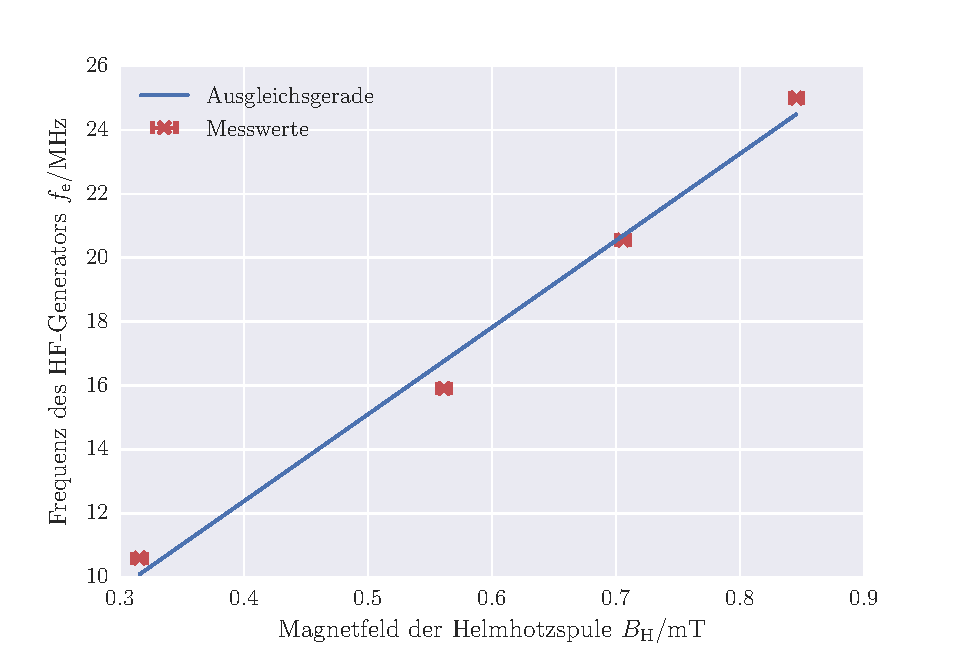
\includegraphics[scale=1]{../Grafiken/Magenetfeld.pdf}
 \caption{Grafische Darstellung der Abhängigkeit der HF-Generator Frequenz von der eingestellten Resonanzmagnetfeldstärke mit lineare Ausgleichsfunktion. \label{fig:magnetfeld}}
 \end{figure} 
\FloatBarrier

Die durchgeführte lineare Regression mit einer Funktion der Form
\begin{empheq}{equation}
	f(B) = a*B + b
\end{empheq}
lieferte die Regressionsparameter 
%a [MHz/T]  27170.5569932 +/- 2031.35133291
%b [MHz]    1.52051720938 +/- 1.29581585756
\addtocounter{equation}{-1}
\begin{subequations}
	\begin{empheq}{align}
	\label{eq:fit_a}
		a &= \SI{27(2)}{\giga\hertz\per\tesla} \\
		b &=  \SI{2(1)}{\mega\hertz}
	\end{empheq}
\end{subequations}

Da die Ausgleichsgerade in \cref{fig:magnetfeld} der Form nach \eqref{eq:energie} entspricht ergibt 
sich für die bestimmte Steigung
\begin{empheq}{align*}
	 a &= g \dfrac{\mu_{\mathrm{B}}}{h}\\ 
	 &= \dfrac{g}{2} \dfrac{e}{m_0} \dfrac{\hbar}{h}.
\end{empheq}
Dadurch erhält man den Wert für den Landé-Faktor des Elektrons durch 
\begin{empheq}{equation}
g = 4\pi\dfrac{m_0}{e} \cdot a
\end{empheq}
Mit der bestimmten Steigung  \eqref{eq:fit_a} ergibt sich für den Landé-Faktor der Wert
\begin{empheq}{equation}
g = \num{1.9(2)}.
\end{empheq}

